\documentclass{article}
\usepackage[utf8]{inputenc}
% For more functions involving bibliography
\usepackage{natbib}
% For typesetting Korean
\usepackage{kotex}
% For typesetting IPA phonetic symbols
\usepackage{tipa}
%For inserting pictures
\usepackage{graphicx}
%For glossing linguistic examples
\usepackage{linguex}
%For inserting trees
\usepackage{tikz-qtree}
%For inserting hyperlinks and such
\usepackage{hyperref}
%For creating multi-columned texts
\usepackage{multicol}
%For creating OT tableaux widely used in phonology
\usepackage{ot-tableau}
%For additional math symbols
\usepackage{stmaryrd}

%Here's an example of how you might create a customized command for your own use -- this one creates a shortcut for denotation brackets in semantics; see problem 3 for its use
\newcommand{\sem}[1]{\ensuremath{\llbracket#1\rrbracket}}

\title{Experimental Linguistics \\ \LaTeX\ Worksheet}
\date{September 2019}

\begin{document}

\maketitle

\noindent Create a document with the following sections, and answer the questions.

\section{Phonetic symbols and IPA}

\begin{enumerate}
    \item Fill in the blank by transcribing your name in IPA and typesetting it in LaTeX. 
    \ex. My name is [\textipa{s\super h2nu}].
    
    The following site may be of help (though beware, it is not always accurate!):
    
    \begin{quotation}
    \noindent 
    \url{http://pronunciation.cs.pusan.ac.kr/}  
    \end{quotation}
    
    \item Fill in the blank with IPA symbols after discussing the problem with your partner. Typeset it in LaTeX.
    
    \ex. Jimin wants to ask Siri to play Spike Jonze's 2013 film, \textit{Her} [\textipa{h@\*r}]. \\
    He forgets that the language setting is in English, 
    and says: 시리야! 헐 [\textipa{h2l}] 
    좀 틀어줘! What do you think happened?
    
\end{enumerate}


\section{Linguistic examples}

\noindent Gloss the following in English with appropriate case markings.

\exg. 나-는 어디-에서 왔-고 무엇-을 하는-가. \\
I-\textsc{nom} where-from come-and what-\textsc{acc} do-\textsc{int}. \\

\section{Pictures, symbols, and trees}

\begin{enumerate}
    \item Draw a syntactic tree for the following sentence using LaTeX.
    
    \ex. Colorless green ideas sleep furiously.
    
    \begin{tikzpicture}
    \tikzset{every tree node/.style={align=center,anchor=north}}
    \Tree 
    [.S [.NP [.Adj\\colorless ]  
        [.NP  [.Adj\\green ] [.N\\ideas ] ] ] 
        [.VP [.V\\sleep ] [.Adv\\furiously ] ]
    ]
    \end{tikzpicture}
    
    Note: I tried the one without vertical lines before the terminal nodes; to implement this customization (and other tweaks), you need to embed your codes in tikzpicture environment as shown above.\ Note also that the above is by no means an informed/sophisticated syntactic tree! 
    
    \item Give the name and the denotation (substitute it with a picture, in lieu of the actual person) of your favorite linguist, author, or celebrity. For example:
    
    \ex.  \sem{Sejong} = 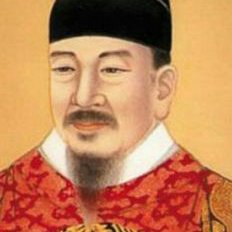
\includegraphics[width=3.4cm]{sejong.jpg} 
    
    Call in \verb \usepackage{graphicx} ~at the preamble, upload the image file you want to include, then use the following command: \\
    \verb \includegraphics[width=3.4cm]{name_of_pic.jpg} ~to include a picture. 
    
\end{enumerate}

\section{Citations and references}

\noindent Search for and find 1 book and 2 journal articles that is relevant to your research project or your main area of interest. Create a .bib file and Cite the references (in author year format) as follows. Create a reference section at the end.

\ex. Today, I read \cite{strand1996}, \cite{johnson2006}, and \cite{eckert2013}. 

\vspace{12pt}


% \begin{center}
% \Large Please turn in the .pdf and the .bib file at the end of the class!
% \end{center}


\bibliographystyle{chicago}
\bibliography{tutorial-bibliography.bib}

\end{document}
